\documentclass{standalone}

\usepackage{tikz}
\usepackage{tkz-euclide}
\usetikzlibrary{calc}
\usetikzlibrary{positioning}
\usetikzlibrary{arrows.meta}

\usepackage{times}


\begin{document}
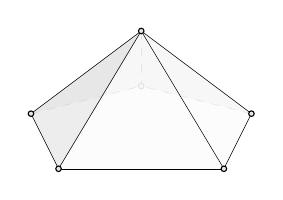
\begin{tikzpicture}[%
  >={Stealth[scale=1.0]},
  scale=3.5
]

  \tkzDefPoint(0.0, 0.3){x}

  \tkzDefPoint(0.4, 0.0){A}
  \tkzDefPoint(0.3, -0.2){B}
  \tkzDefPoint(-0.3, -0.2){C}
  \tkzDefPoint(-0.4, 0.0){D}
  \tkzDefPoint(0.0, 0.1){E}

  \tkzFillPolygon[color=black!20](x,D,E)
  \tkzFillPolygon[color=black!20](x,E,A)
  \tkzDrawSegments[dashed](x,E A,E D,E)
  \tkzDrawPoints(E)

  \tkzFillPolygon[color=black!1,opacity=0.9](x,B,C)
  \tkzFillPolygon[color=black!1,opacity=0.9](x,A,B)
  \tkzFillPolygon[color=black!8,opacity=0.9](x,C,D)

  % \tkzDefPointOnLine[pos=0.5](x,A)\tkzGetPoint{tmp}
  % \tkzFillCircle[color=black!10,opacity=0.5,R](x)
  % \tkzDrawCircle[black,dashed,fill=black!10,opacity=0.8](x,tmp)
  % \tkzFillSector[R with nodes,fill=black!10,opacity=0.5](x,0.5)(B,A)
  % \tkzDrawArc[R with nodes,dashed](x,0.5)(B,D)
  % \tkzDrawArc[R with nodes,dashed](x,0.5)(D,A)

  \tkzDrawSegments(x,A x,B x,C x,D)
  \tkzDrawSegments(A,B B,C C,D)
  \tkzDrawPoints(x,A,B,C,D)

\end{tikzpicture}
\end{document}
